%%
%% getstart.tex -- Flight Gear documentation: Installation and Getting Started
%% Chapter file
%%
%% Copyright (C) 2002 Michael Basler
%%                  & Bernhard Buckel
%%
%% This program is free software; you can redistribute it and/or
%% modify it under the terms of the GNU General Public License as
%% published by the Free Software Foundation; either version 2 of the
%% License, or (at your option) any later version.
%%
%% This program is distributed in the hope that it will be useful, but
%% WITHOUT ANY WARRANTY; without even the implied warranty of
%% MERCHANTABILITY or FITNESS FOR A PARTICULAR PURPOSE.  See the GNU
%% General Public License for more details.
%%
%% You should have received a copy of the GNU General Public License
%% along with this program; if not, write to the Free Software
%% Foundation, Inc., 675 Mass Ave, Cambridge, MA 02139, USA.
%%
%% $Id: takeof.tex,v 0.6 2002/09/09 michael
%% (Log is kept at end of this file)

%%%%%%%%%%%%%%%%%%%%%%%%%%%%%%%%%%%%%%%%%%%%%%%%%%%%%%%%%%%%%%%%%%%%%%%%%%%%%%%%%%%%%%%%%%%%%%%
\chapter{Takeoff: How to start the program\label{takeoff}}
%%%%%%%%%%%%%%%%%%%%%%%%%%%%%%%%%%%%%%%%%%%%%%%%%%%%%%%%%%%%%%%%%%%%%%%%%%%%%%%%%%%%%%%%%%%%%%%
\markboth{\thechapter.\hspace*{1mm}
TAKEOFF}{\thesection\hspace*{1mm} Command line parameters}
%%%%%%%%%%%%%%%%%%%%%%%%%%%%%%%%%%%%%%%%%%%%%%%%%%%%%%%%%%%%%%%%%%%%%%%%%%%%%%%%%%%%%%%%%%%%%%%
\section{Launching the simulator under Unix/Linux}\index{Launching Flightgear!Linux}\index{Starting Flightgear!Linux}
%%%%%%%%%%%%%%%%%%%%%%%%%%%%%%%%%%%%%%%%%%%%%%%%%%%%%%%%%%%%%%%%%%%%%%%%%%%%%%%%%%%%%%%%%%%%%%%

\centerline{\fbox{
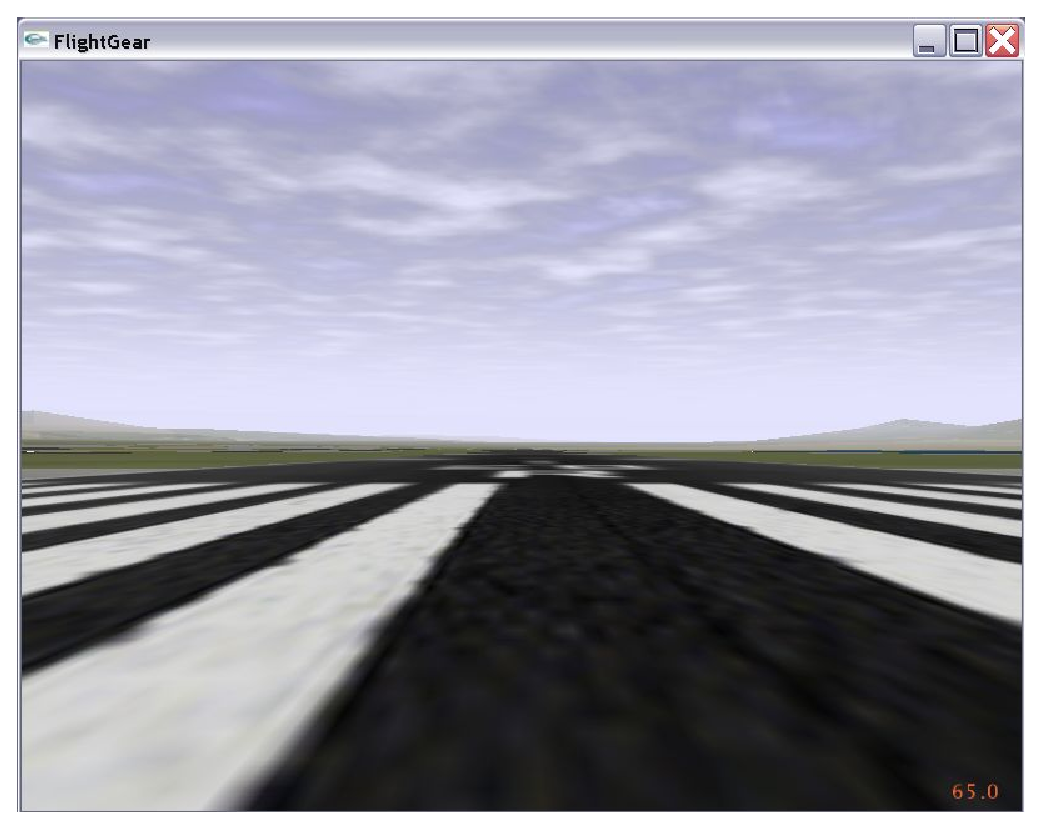
\includegraphics[clip,width=12.5cm]{ksfo}
}}
\smallskip

 \noindent
Fig.\,3: \textit{Ready for takeoff. Waiting at the default startup position at San
Francisco Itl., KSFO.}
\medskip

Before you can run \FlightGear{}, you need to have a couple of environmental variables set.

\begin{itemize}
\item You must add \texttt{/usr/local/FlightGear/lib} to your \texttt{LD\_LIBRARY\_PATH}
\item \texttt{FG\_HOME} must be set to the root of your \FlightGear{} installation. e.g. \texttt{/usr/local/FlightGear}.
\item \texttt{FG\_ROOT} must be set to the date directory of your \FlightGear{} installation. e.g. \texttt{/usr/local/FlightGear/data}.
\item \texttt{FG\_SCENERY} should be a list of scenery directories, separated by '':''. This works like \texttt{PATH} when searching for scenery. e.g. \texttt{\$FG\_HOME/Scenery:\$FG\_ROOT/Scenery:\$FG\_ROOT/WorldScenery}.
\end{itemize}

\noindent
To add these in the Bourne shell (and compatibles):
\begin{verbatim}
LD_LIBRARY_PATH=/usr/local/FlightGear/lib:$LD_LIBRARY_PATH
export LD_LIBRARY_PATH
FG_HOME=/usr/local/FlightGear
export FG_HOME
FG_ROOT=/usr/local/FlightGear/data
export FG_ROOT
FG_SCENERY=$FG_HOME/Scenery:$FG_ROOT/Scenery:$FG_ROOT/WorldScenery
export FG_SCENERY
\end{verbatim}
\noindent
 or in C shell (and compatibles):
\begin{verbatim}
setenv LD_LIBRARY_PATH=/usr/local/FlightGear/lib:$LD_LIBRARY_PATH
setenv FG_HOME=/usr/local/FlightGear
setenv FG_ROOT=/usr/local/FlightGear/data
setenv FG_SCENERY=$FG_HOME/Scenery:$FG_ROOT/Scenery:$FG_ROOT/WorldScenery
\end{verbatim}
Once you have these environmental variables set up, simply start \FlightGear{} by running
\texttt{fgfs -$ $-option1 -$ $-option2\dots}.
\medskip
Command-line options are described in Chapter~\ref{options}.

%%%%%%%%%%%%%%%%%%%%%%%%%%%%%%%%%%%%%%%%%%%%%%%%%%%%%%%%%%%%%%%%%%%%%%%%%%%%%%%%%%%%%%%%%%%%%%%
\section{Launching the simulator under Windows}\index{Launching Flightgear!Windows}\index{Starting Flightgear!Windows}
%%%%%%%%%%%%%%%%%%%%%%%%%%%%%%%%%%%%%%%%%%%%%%%%%%%%%%%%%%%%%%%%%%%%%%%%%%%%%%%%%%%%%%%%%%%%%%%
The pre-built windows binaries come complete with a graphical wizard to start \FlightGear{}. Simply double-click on the \texttt{FlightGear Launcher} Start Menu item, or the icon on the Desktop. The launcher allows you to select
\begin{itemize}
\item your aircraft
\item the start airport and runway
\item time of day
\item current weather
\item \dots{} and whole lot of other environmental settings
\end{itemize}

 \centerline{\fbox{
\includegraphics[clip,width=12.5cm]{launcher}
}}
\smallskip

 \noindent
Fig.\,4: \textit{The FlightGear Launcher}
\medskip

Alternatively, you can run FlightGear from the command line. Open
a command shell, change to the directory where your binary resides
(typically something like \texttt{c:/FlightGear/Win32/bin} where you might have to substitute
\texttt{c:/FlightGear} in favor of your \FlightGear{} directory), set the \Index{environment variables} by typing 
\medskip

\begin{verbatim}
SET FG_HOME=c:\FlightGear
SET FG_ROOT=c:\FlightGear\data
SET FG_SCENERY=c:\FlightGear\scenery;c:\FlightGear\data\Scenery
\end{verbatim}
\medskip

\noindent
 and invoke \FlightGear{} (within the same Command shell, as environment
 settings are only valid locally within the same shell) via
  \medskip

\texttt{fgfs -$ $-option1 -$ $-option2\dots}.
 \medskip

Of course, you can create a batch fiile with Windows \texttt{Editor} using the
lines above.

For getting maximum performance it is recommended to minimize (iconize) the text output
window while running \FlightGear{}.

%%%%%%%%%%%%%%%%%%%%%%%%%%%%%%%%%%%%%%%%%%%%%%%%%%%%%%%%%%%%%%%%%%%%%%%%%%%%%%%%%%%%%%%%%%%%%%%
\section{Launching the simulator under Mac OS X}\index{Launching Flightgear!Mac OS X}\index{Starting Flightgear!Mac OS X}
%%%%%%%%%%%%%%%%%%%%%%%%%%%%%%%%%%%%%%%%%%%%%%%%%%%%%%%%%%%%%%%%%%%%%%%%%%%%%%%%%%%%%%%%%%%%%%%
Say, you downloaded the base package and binary to your home directory. Then you can open \texttt{Terminal.app} and execute the following sequence:
\medskip

\noindent
\texttt{setenv FG\_ROOT ~/fgfs-base-X.X.X \./fgfs-X.X.X.-date}\\
\texttt{-$ $-option1 -$ $- option 2} (one line)
\medskip

\noindent
or
\medskip

\noindent
\texttt{./fgfs-X.X.X-version-date}
 \texttt{-$ $-fg-root=\~/fgfs-base-X.X.X}\\
 \texttt{-$ $-option1 -$ $-option2}. (one line)

%%%%%%%%%%%%%%%%%%%%%%%%%%%%%%%%%%%%%%%%%%%%%%%%%%%%%%%%%%%%%%%%%%%%%%%%%%%%%%%%%%%%%%%%%%%%%%%
\section{Command line parameters\label{options}}\index{command line options}
%%%%%%%%%%%%%%%%%%%%%%%%%%%%%%%%%%%%%%%%%%%%%%%%%%%%%%%%%%%%%%%%%%%%%%%%%%%%%%%%%%%%%%%%%%%%%%%
Following is a complete list and short description of the numerous \Index{command line options}
available for \FlightGear{}\. Most of these options are exposed through the FlightGear launcher delivered with the
Windows binaries.

If you have options you re-use continually, you can include them in a preferences file. As it depends on your
\Index{preferences}, it is not delivered with \FlightGear{}, but can be created with any text editor (notepad, emacs, vi, if you like). 

\begin{itemize}
\item On Unix systems, create a \texttt{.fgfsrc}\index{.fgfsrc} file in your home directory.
\item On Windows, create a \texttt{system.fgfsrc},\index{system.fgfsrc} in
the top \texttt{FG\_ROOT} directory (e.g. \texttt{c:\\FlightGear}). 
\end{itemize}

%%%%%%%%%%%%%%%%%%%%%%%%%%%%%%%%%%%%%%%%%%%%%%%%%%%%%%%%%%%%%%%%%%%%%%%%%%%%%%%%%%%%%%%%%%%%%%%
\subsection{General Options}\index{options!general}\label{generaloptions}
%%%%%%%%%%%%%%%%%%%%%%%%%%%%%%%%%%%%%%%%%%%%%%%%%%%%%%%%%%%%%%%%%%%%%%%%%%%%%%%%%%%%%%%%%%%%%%%
\begin{itemize}
\item{\texttt{-$ $-help}}: Shows the most relevant command line options only.
\item{\texttt{-$ $-help} \texttt{-verbose}}: Shows all command line options.
\item{\texttt{-$ $-fg-root={\it path}}}: Tells \FlightGear{} where to look for its root data
  files if you didn't compile it with the \Index{default settings}.
\item{\texttt{-$ $-fg-scenery={\it path}}}: Allows specification of a path to the base scenery path \index{scenery directory!path}, in case scenery is not at the default position under\\
 \texttt{\$FG\underline{~}ROOT/Scenery}; this might be especially useful in case you
have scenery on a CD-ROM.
\item{\texttt{-$ $-disable-game-mode}}: Disables \Index{full screen display}.
\item{\texttt{-$ $-enable-game-mode}}: Enables full screen display.
\item{\texttt{-$ $-disable-splash-screen}}: Turns off the rotating 3DFX logo
 when the accelerator board gets initialized (3DFX only).
\item{\texttt{-$ $-enable-splash-screen}}: If you like advertising, set this!
\item{\texttt{-$ $-disable-intro-music}}: No audio sample is being played when
  \FlightGear{} starts up. Suggested in case of trouble with playing the intro.
\item{\texttt{-$ $-enable-intro-music}}: If your machine is powerful enough, enjoy
  this setting.
\item{\texttt{-$ $-disable-mouse-pointer}}: Disables extra \Index{mouse pointer}.
\item{\texttt{-$ $-enable-mouse-pointer}}: Enables extra \Index{mouse pointer}. Useful in
full screen mode for old Voodoo based cards.
\item{\texttt{-$ $-enable-random-objects}}: Include random scenery objects (buildings/trees). This is the default.
\item{\texttt{-$ $-disable-random-objects}}: Exclude random scenery objects (buildings/trees).
\item{\texttt{-$ $-disable-freeze}}: This will put you into \FlightGear{} with the
  engine running, ready for Take-Off.
\item{\texttt{-$ $-enable-freeze}}: Starts \FlightGear{} in \Index{frozen state}.
\item{\texttt{-$ $-disable-fuel-freeze}}: Fuel is consumed normally.
\item{\texttt{-$ $-enable-fuel-freeze}}: Fuel tank quantity is forced to remain constant.
\item{\texttt{-$ $-disable-clock-freeze}}: Time of day advances normally.
\item{\texttt{-$ $-enable-clock-freeze}}: Do not advance time of day.
\item{\texttt{-$ $-control-mode}}: Specify your \Index{control device} (\Index{joystick},
 keyboard, mouse) Defaults to \Index{joystick} (\Index{yoke}).
\item{\texttt{-$ $-disable-auto-coordination}}: Switches \Index{auto coordination} between
aileron/rudder off (default).
\item{\texttt{-$ $-enable-auto-coordination}}: Switches auto coordination between
aileron/rudder on (recommended without pedals).
\item{\texttt{-$ $-browser-app=/path/to/app}}:  specify location of your web browser. Example:
\texttt{-$ $-browser-app=}\\  \texttt{''C:$\backslash$Program~Files$\backslash$Internet~Explorer$\backslash$iexplore.exe''} (Note the '' '' because of the spaces!).
\item{\texttt{-$ $-prop:name=value:}}  set property \texttt{name} to \texttt{value}\\Example:
\texttt{-$ $-prop:/engines/engine0/running=true} for starting with running engines. Another example:\\
\texttt{-$ $-aircraft=c172}\\
\texttt{-$ $-prop:/consumables/fuels/tank[0]/level-gal=10}\\
\texttt{-$ $-prop:/consumables/fuels/tank[1]/level-gal=10}\\
filles the Cessna for a short flight.
\item{\texttt{-$ $-config=path:}}  Load additional properties from the given path. Example: \texttt{runfgfs -$ $-config=./Aircraft/X15-set.xml}
\item{\texttt{-$ $-units-feet}}: Use feet for distances.
\item{\texttt{-$ $-units-meters}}: Use meters for distances.
\end{itemize}
%%%%%%%%%%%%%%%%%%%%%%%%%%%%%%%%%%%%%%%%%%%%%%%%%%%%%%%%%%%%%%%%%%%%%%%%%%%%%%%%%%%%%%%%%%%%%%%
\subsection{Features}\index{options!features}
%%%%%%%%%%%%%%%%%%%%%%%%%%%%%%%%%%%%%%%%%%%%%%%%%%%%%%%%%%%%%%%%%%%%%%%%%%%%%%%%%%%%%%%%%%%%%%%
\begin{itemize}
\item{\texttt{-$ $-disable-hud}}: Switches off the \Index{HUD} (\textbf{H}ead \textbf{U}p
  \textbf{D}isplay).
\item{\texttt{-$ $-enable-hud}}: Turns the  \Index{HUD} on.
\item{\texttt{-$ $-enable-anti-aliased-hud}}: Turns on \Index{anti-aliaseded HUD lines} for better quality,
if hardware supports this.
\item{\texttt{-$ $-disable-anti-aliased-hud}}: Turns off anti-aliaseded HUD lines.
\item{\texttt{-$ $-enable-panel}}: Turns the \Index{instrument panel} on (default).
\item{\texttt{-$ $-disable-panel}}: Turns the \Index{instrument panel} off.
\item{\texttt{-$ $-disable-sound}}: Self explaining.
\item{\texttt{-$ $-enable-sound}}: See above.
\end{itemize}

%%%%%%%%%%%%%%%%%%%%%%%%%%%%%%%%%%%%%%%%%%%%%%%%%%%%%%%%%%%%%%%%%%%%%%%%%%%%%%%%%%%%%%%%%%%%%%%
\subsection{Aircraft\index{aircraft!selection}}\index{options!aircraft}
%%%%%%%%%%%%%%%%%%%%%%%%%%%%%%%%%%%%%%%%%%%%%%%%%%%%%%%%%%%%%%%%%%%%%%%%%%%%%%%%%%%%%%%%%%%%%%%

\begin{itemize}
\item{\texttt{-$ $-aircraft={\it name of aircraft definition file}}} Example: \texttt{-$ $-aircraft=c310}. For possible choices check the directory \texttt{/FlightGear/Aircraft}. Do not include the extension \texttt{''-set.xml''} into the aircraft name but use the remaining beginning of the respective file names for choosing an aircraft. This way flight model, panel etc\. are all loaded in a consistent way. For a full list, see Sec.~\ref{hangar} below.
\item{\texttt{-$ $-show-aircraft}}: Print a sorted list of the currently available aircraft types. 
\end{itemize}

%%%%%%%%%%%%%%%%%%%%%%%%%%%%%%%%%%%%%%%%%%%%%%%%%%%%%%%%%%%%%%%%%%%%%%%%%%%%%%%%%%%%%%%%%%%%%%%
\subsection{Flight model\index{flight dynamics model}}\index{options!flight model}\label{flight dynamics model}
%%%%%%%%%%%%%%%%%%%%%%%%%%%%%%%%%%%%%%%%%%%%%%%%%%%%%%%%%%%%%%%%%%%%%%%%%%%%%%%%%%%%%%%%%%%%%%%
\begin{itemize}
\item{\texttt{-$ $-fdm={\it abcd}}} Select the core \Index{flight model}.
Options are \texttt{jsb, larcsim, yasim, magic, balloon, external, pipe, ada, null}. Default value is
\texttt{jsb} (\JSBSim)\index{JSBSim}. larcsim is the flight model which
\FlightGear{} inherited from the LaRCSim simulator\. yasim is Any Ross' Yet
Another Flight Dynamics Simulator. Magic is a slew mode (which drives the
UFO aircraft). Balloon is a hot air balloon. External refers to remote
control of the simulator via TCP socket, pipe is for local control via named
pipe. Null selects no flight dynamics model at all. The \Index{UIUC flight
model} is not chosen this way but via the next option! For further
information on flight models cf. Section~\ref{flightmodels} and below.
\item{\texttt{-$ $-aero={\it abcd}}} Specifies the \Index{aircraft model} to load. Default is a Cessna c172. Alternatives available depend on the flight model chosen. 
\item{\texttt{-$ $-model-hz={\it n}}} Run the Flight Dynamics Model with this rate
(iterations per second).
\item{\texttt{-$ $-speed={\it n}}} Run the Flight Dynamics Model this much faster than real
time.
\item{\texttt{-$ $-notrim}} Do NOT attempt to trim the model when initializing JSBSim.
\item{\texttt{-$ $-on-ground}}: Start up at ground level (default).
\item{\texttt{-$ $-in-air}}: Start up in the air. Naturally, you have to specify an
initial altitude as below for this to make sense. This is a must for the X15.
\item{\texttt{-$ $-wind={\it DIR@SPEED}}}: Specify wind coming from the direction DIR (in
degrees) at speed SPEED (knots). Values may be specified as a range by using a clon separator; e.g. 180:220@10:15
\item{\texttt{-$ $-random-wind}}: Adds random wind to make flying more challenging
\end{itemize}

%%%%%%%%%%%%%%%%%%%%%%%%%%%%%%%%%%%%%%%%%%%%%%%%%%%%%%%%%%%%%%%%%%%%%%%%%%%%%%%%%%%%%%%%%%%%%%%
\subsection{Initial Position and Orientation\label{aiportid}}\index{options!initial position}\index{options!orientation}
%%%%%%%%%%%%%%%%%%%%%%%%%%%%%%%%%%%%%%%%%%%%%%%%%%%%%%%%%%%%%%%%%%%%%%%%%%%%%%%%%%%%%%%%%%%%%%%
\begin{itemize}
\item{\texttt{-$ $-airport-id={\it ABCD}}}: If you want to start directly at an \Index{airport},
  enter its international code,\index{airport code} i.e. KJFK for JFK airport in New York etc.
  A long/short list of the IDs of the airports being implemented can
  be found in \texttt{/Flight Gear/Airports}. You only have to unpack
  one of the files with \texttt{gunzip}. Keep in mind, you need the
  terrain data for the relevant region, though!\index{airport code}
\item{\texttt{-$ $-offset-distance={\it nm}}}: Here you can specify the distance to
threshold in nm.
\item{\texttt{-$ $-offset-azimuth={\it deg}}}: Here you can specify the heading to
threshold in degrees.
\item{\texttt{-$ $-lon={\it degrees}}}: This is the \Index{startup longitude} in degrees (west =
-).
\item{\texttt{-$ $-lat={\it degrees}}}: This is the \Index{startup latitude} in degrees (south =
-).
\item{\texttt{-$ $-altitude={\it feet}}}: This is useful if you want to start in free
flight in connection with \texttt{-$ $-in-air}. Altitude specified in feet unless you
choose \texttt{-$ $-units-meters}.
\item{\texttt{-$ $-heading={\it degrees}}}: Sets the \Index{initial heading} (yaw angle) in degrees.
\item{\texttt{-$ $-roll={\it degrees}}}: Sets the \Index{startup roll angle} (roll angle) in degrees.
\item{\texttt{-$ $-pitch={\it degrees}}}: Sets the \Index{startup pitch angle} (pitch angle) in degrees.
\item{\texttt{-$ $-uBody={\it feet per second}}}: Speed along the body X axis in feet per second, unless you
choose \texttt{-$ $-units-meters}.
\item{\texttt{-$ $-vBody={\it feet per second}}}: Speed along the body Y axis in feet per second, unless you
choose \texttt{-$ $-units-meters}.
\item{\texttt{-$ $-wBody={\it feet per second}}}: Speed along the body Z axis in feet per second, unless you
choose \texttt{-$ $-units-meters}.
\item{\texttt{-$ $-vc={\it knots}}}: Allows specifying the initial airspeed in knots
(only in connection with  \texttt{-$ $-fdm=jsb}).
\item{\texttt{-$ $-mach={\it num}}}: Allows specifying the initial airspeed as Mach
number (only in connection with  \texttt{-$ $-fdm=jsb}).
\item{\texttt{-$ $-glideslope={\it degrees}}}: Allows specifying the flight path angle (can be positive).
\item{\texttt{-$ $-roc={\it fpm}}}: Allows specifying the initial climb rate (can be negative).
\end{itemize}
%%%%%%%%%%%%%%%%%%%%%%%%%%%%%%%%%%%%%%%%%%%%%%%%%%%%%%%%%%%%%%%%%%%%%%%%%%%%%%%%%%%%%%%%%%%%%%%
\subsection{Rendering Options\index{options!rendering}}
%%%%%%%%%%%%%%%%%%%%%%%%%%%%%%%%%%%%%%%%%%%%%%%%%%%%%%%%%%%%%%%%%%%%%%%%%%%%%%%%%%%%%%%%%%%%%%%
\begin{itemize}
\item{\texttt{-$ $-bpp={\it depth}}}: Specify the bits per pixel.
\item{\texttt{-$ $-fog-disable}}: To cut down the rendering efforts, distant
  regions are vanishing in \Index{fog} by default. If you disable \Index{fog}ging,
  you'll see farther but your frame rates will drop.
\item{\texttt{-$ $-fog-fastest}}: The scenery will not look very nice but
  \Index{frame rate} will increase.
\item{\texttt{-$ $-fog-nicest}}: This option will give you a fairly realistic
  view of flying on a hazy day.\index{haze}
\item{\texttt{-$ $-enable-clouds}}: Enable \Index{cloud layer} (default).
\item{\texttt{-$ $-disable-clouds}}: Disable cloud layer.
\item{\texttt{-$ $-fov={\it degrees}}}: Sets the \Index{field of view} in degrees.
Default is 55.0.
\item{\texttt{-$ $-disable-fullscreen}}: Disable \Index{full screen mode} (default).
\item{\texttt{-$ $-enable-fullscreen}}: Enable full screen mode.
\item{\texttt{-$ $-shading-flat}}: This is the fastest mode but the terrain will look ugly!
This option might help if your video processor is really slow.
\item{\texttt{-$ $-shading-smooth}}: This is the recommended (and default) setting - things will look really nice.
\item{\texttt{-$ $-disable-skyblend}}: No fogging or \Index{haze}, sky will be displayed
  using just one color. Fast but ugly!
\item{\texttt{-$ $-enable-skyblend}}: Fogging/haze is enabled, sky and \Index{terrain} look realistic. This is the default and recommended setting.
\item{\texttt{-$ $-disable-textures}}: Terrain details will be disabled. Looks ugly, but might help if your video board is slow.
\item{\texttt{-$ $-enable-textures}}: Default and recommended.
\item{\texttt{-$ $-enable-wireframe}}: If you want to know how the world of \FlightGear{} looks like internally, try
this!\index{wireframe}
\item{\texttt{-$ $-disable-wireframe}}: No wireframe. Default.
\item{\texttt{-$ $-geometry={\it WWWxHHH}}}: Defines the size of the window used, i.e.
\texttt{WWWxHHH} can be \texttt{640x480}, \texttt{800x600}, or
\texttt{1024x768}.\index{window size}
\item{\texttt{-$ $-view-offset={\it xxx}}}: Allows setting the default forward view direction as an offset from straight
ahead. Possible values are \texttt{LEFT, RIGHT, CENTER}, or a specific number of degrees.
Useful for multi-window display.\index{offset}
\item{\texttt{-$ $-visibility={\it meters}}}: You can specify the initial visibility in meters here.
\item{\texttt{-$ $-visibility-miles={\it miles}}}: You can specify the initial visibility in miles here.
\end{itemize}

%%%%%%%%%%%%%%%%%%%%%%%%%%%%%%%%%%%%%%%%%%%%%%%%%%%%%%%%%%%%%%%%%%%%%%%%%%%%%%%%%%%%%%%%%%%%%%%
\subsection{HUD Options\index{HUD}\index{options!HUD}}
%%%%%%%%%%%%%%%%%%%%%%%%%%%%%%%%%%%%%%%%%%%%%%%%%%%%%%%%%%%%%%%%%%%%%%%%%%%%%%%%%%%%%%%%%%%%%%%
\begin{itemize}
\item{\texttt{-$ $-hud-tris}}: HUD displays the number of \Index{triangles} rendered.
\item{\texttt{-$ $-hud-culled}}: HUD displays percentage of triangles culled.
\end{itemize}
%%%%%%%%%%%%%%%%%%%%%%%%%%%%%%%%%%%%%%%%%%%%%%%%%%%%%%%%%%%%%%%%%%%%%%%%%%%%%%%%%%%%%%%%%%%%%%%
\subsection{Time Options}\index{time options}\index{options!time}
%%%%%%%%%%%%%%%%%%%%%%%%%%%%%%%%%%%%%%%%%%%%%%%%%%%%%%%%%%%%%%%%%%%%%%%%%%%%%%%%%%%%%%%%%%%%%%%
\begin{itemize}
\item{\texttt{-$ $-time-offset={\it [+-]hh:mm:ss}}}: Offset local \Index{time} by this amount.
\item{\texttt{-$ $-time-match-real}}: Synchronize real-world and \FlightGear{} time.
\item{\texttt{-$ $-time-match-local}}: Synchronize local real-world and \FlightGear{} time.
\item{\texttt{-$ $-start-date-sys={\it yyyy:mm:dd:hh:mm:ss}}}: Specify a \Index{starting time} and date. Uses your system time.
\item{\texttt{-$ $-start-date-gmt={\it yyyy:mm:dd:hh:mm:ss}}}: Specify a starting time and
date. Time is Greenwich Mean Time.
\item{\texttt{-$ $-start-date-lat={\it yyyy:mm:dd:hh:mm:ss}}}: Specify a starting time and
date. Uses local aircraft time.
\end{itemize}
%%%%%%%%%%%%%%%%%%%%%%%%%%%%%%%%%%%%%%%%%%%%%%%%%%%%%%%%%%%%%%%%%%%%%%%%%%%%%%%%%%%%%%%%%%%%%%%
\subsection{Network Options}\index{network options}\index{options!network}
%%%%%%%%%%%%%%%%%%%%%%%%%%%%%%%%%%%%%%%%%%%%%%%%%%%%%%%%%%%%%%%%%%%%%%%%%%%%%%%%%%%%%%%%%%%%%%%
\begin{itemize}
\item{\texttt{-$ $-httpd={\it port}}}: Enable \Index{http server} on the specified port.
\item{\texttt{-$ $-telnet={\it port}}}: Enable \Index{telnet server} on the specified port.
\item{\texttt{-$ $-jpg-httpd={\it port}}}: Enable screen shot http server on the specified port.
\item{\texttt{-$ $-enable-network-olk}}: Enables Oliver Delises's multi-pilot mode.
\item{\texttt{-$ $-disable-network-olk}}: Disables Oliver Delises's multi-pilot mode (default).
\item{\texttt{-$ $-net-hud}}: HUD displays network info.
\item{\texttt{-$ $-net-id={\it name}}}: Specify your own \Index{callsign}
 \end{itemize}
%%%%%%%%%%%%%%%%%%%%%%%%%%%%%%%%%%%%%%%%%%%%%%%%%%%%%%%%%%%%%%%%%%%%%%%%%%%%%%%%%%%%%%%%%%%%%%%
\subsection{Route/Waypoint Options}\index{options!route}\index{options!waypoint}
%%%%%%%%%%%%%%%%%%%%%%%%%%%%%%%%%%%%%%%%%%%%%%%%%%%%%%%%%%%%%%%%%%%%%%%%%%%%%%%%%%%%%%%%%%%%%%%
\begin{itemize}
\item{\texttt{-$ $-wp={\it ID[@alt]}}}: Allows specifying a waypoint for the GC autopilot; it
is possible to specify multiple waypoints (i.e\. a route) via multiple instances of this
command.
\item{\texttt{-$ $-flight-plan={\it [file]}}}: This is more comfortable if
you have several waypoints. You can  specify a file to read them from.
\end{itemize}

Note: These options are rather geared to the advanced user who knows what he is doing. 

%%%%%%%%%%%%%%%%%%%%%%%%%%%%%%%%%%%%%%%%%%%%%%%%%%%%%%%%%%%%%%%%%%%%%%%%%%%%%%%%%%%%%%%%%%%%%%%
\subsection{IO Options}\index{options!IO}
%%%%%%%%%%%%%%%%%%%%%%%%%%%%%%%%%%%%%%%%%%%%%%%%%%%%%%%%%%%%%%%%%%%%%%%%%%%%%%%%%%%%%%%%%%%%%%%
\begin{itemize}
\item{\texttt{-$ $-garmin={\it params}}}: Open connection using the Garmin GPS protocol.
\item{\texttt{-$ $-joyclient={\it params}}}: Open connection to an Agwagon joystick.
\item{\texttt{-$ $-native-ctrls={\it params}}}: Open connection using the FG native Controls protocol.
\item{\texttt{-$ $-native-fdm={\it params}}}: Open connection using the FG Native FDM protocol.
\item{\texttt{-$ $-native={\it params}}}: Open connection using the FG Native protocol.
\item{\texttt{-$ $-nmea={\it params}}}: Open connection using the NMEA protocol.
\item{\texttt{-$ $-opengc={\it params}}}: Open connection using the OpenGC protocol.
\item{\texttt{-$ $-props={\it params}}}: Open connection using the interactive property manager.
\item{\texttt{-$ $-pve={\it params}}}: Open connection using the PVE protocol.
\item{\texttt{-$ $-ray={\it params}}}: Open connection using the RayWoodworth motion chair protocol.
\item{\texttt{-$ $-rul={\it params}}}: Open connection using the RUL protocol.
\item{\texttt{-$ $-atc610x}}: Enable atc610x interface.
\end{itemize}

%%%%%%%%%%%%%%%%%%%%%%%%%%%%%%%%%%%%%%%%%%%%%%%%%%%%%%%%%%%%%%%%%%%%%%%%%%%%%%%%%%%%%%%%%%%%%%%
\subsection{Debugging options}\index{options!debugging}
%%%%%%%%%%%%%%%%%%%%%%%%%%%%%%%%%%%%%%%%%%%%%%%%%%%%%%%%%%%%%%%%%%%%%%%%%%%%%%%%%%%%%%%%%%%%%%%
\begin{itemize}
\item{\texttt{-$ $-trace-read={\it params}}}: Trace the reads for a property; multiple instances are allowed.
\item{\texttt{-$ $-trace-write={\it params}}}: Trace the writes for a property; multiple instances are allowed.
\end{itemize}



%%%%%%%%%%%%%%%%%%%%%%%%%%%%%%%%%%%%%%%%%%%%%%%%%%%%%%%%%%%%%%%%%%%%%%%%%%%%%%%%%%%%%%%%%%%%%%%
\section{Joystick support\label{joysticksupp}}\index{joystick}
%%%%%%%%%%%%%%%%%%%%%%%%%%%%%%%%%%%%%%%%%%%%%%%%%%%%%%%%%%%%%%%%%%%%%%%%%%%%%%%%%%%%%%%%%%%%%%%
Could you imagine a pilot in his or her Cessna controlling the machine with
a keyboard alone? For getting the proper feeling of flight you will need a
joystick/yoke plus rudder pedals, right? However, the combination of
numerous types of \Index{joystick}s, flightsticks, \Index{yoke}s,
\Index{pedal}s etc\. on the market with the several target operating systems,
makes joystick support a nontrivial task in \FlightGear{}.

Beginning with version 0.8.0, \FlightGear{} has a reworked integrated
joystick support, which automatically detects any joystick, yoke, or pedals
attached. Just try it! If this does work for you, lean back and be happy!

Unfortunately, given the several combinations of operating systems supported
by \FlightGear{} (possibly in foreign languages) and joysticks available,
chances are your joystick does not work out of the box. Basically, there are
two alternative approaches to get it going, with the first one being
preferred.


%%%%%%%%%%%%%%%%%%%%%%%%%%%%%%%%%%%%%%%%%%%%%%%%%%%%%%%%%%%%%%%%%%%%%%%%%%%%%%%%%%%%%%%%%%%%%%%
\subsection{Built-in joystick support\label{joystickbuiltin}}\index{options!joystick}
%%%%%%%%%%%%%%%%%%%%%%%%%%%%%%%%%%%%%%%%%%%%%%%%%%%%%%%%%%%%%%%%%%%%%%%%%%%%%%%%%%%%%%%%%%%%%%%

%%%%%%%%%%%%%%%%%%%%%%%%%%%%%%%%%%%%%%%%%%%%%%%%%%%%%%%%%%%%%%%%%%%%%%%%%%%%%%%%%%%%%%%%%%%%%%%
\subsubsection{General remarks\label{generalremarks}}
%%%%%%%%%%%%%%%%%%%%%%%%%%%%%%%%%%%%%%%%%%%%%%%%%%%%%%%%%%%%%%%%%%%%%%%%%%%%%%%%%%%%%%%%%%%%%%%
In order for joystick auto-detection to work, a joystick bindings xml file
must exist for each joystick. This file describes what axes and buttons are
to be used to control which functions in \FlightGear{}.  The associations
between functions and axes or buttons are called ``bindings''.  This
bindings file can have any name as long as a corresponding entry exists in
the joysticks description file
\medskip

     	\texttt{/FlightGear/joysticks.xml} 
\medskip

\noindent
which tells \FlightGear{} where to look for all the bindings files.  We will
look at examples later.

\FlightGear{} includes several such bindings files for several joystick
manufacturers in folders named for each manufacturer.  For example, if you
have a CH Products joystick, look in the folder
\medskip

    \texttt{/FlightGear/Input/Joysticks/CH}
    \medskip
    
\noindent
for a file that might work for your joystick.  If such a file exists and
your joystick is working with other applications, then it should work with
\FlightGear{} the first time you run it.  If such a file does not exist,
then we will discuss in a later section how to create such a file by cutting
and pasting bindings from the examples that are included with \FlightGear{}.

%%%%%%%%%%%%%%%%%%%%%%%%%%%%%%%%%%%%%%%%%%%%%%%%%%%%%%%%%%%%%%%%%%%%%%%%%%%%%%%%%%%%%%%%%%%%%%%
\subsubsection{Verifying your joystick is working\label{verifying}}
%%%%%%%%%%%%%%%%%%%%%%%%%%%%%%%%%%%%%%%%%%%%%%%%%%%%%%%%%%%%%%%%%%%%%%%%%%%%%%%%%%%%%%%%%%%%%%%
Does your computer see your joystick?  One way to answer this question under Linux is to reboot your system and immediately enter on the command line
\medskip

	\texttt{dmesg | grep Joystick}
\medskip

\noindent
which pipes the boot message to grep which then prints every line in the
boot message that contains the string ``Joystick''.  When you do this with a
Saitek joystick attached, you will see a line similar to this one:
\medskip

\begin{ttfamily}
\noindent
   input0: USB HID v1.00 Joystick [SAITEK CYBORG 3D USB] on usb2:3.0
\end{ttfamily}
\medskip

\noindent
This line tells us that a joystick has identified itself as SAITEK CYBORG 3D USB to the operating system.  It does not tell us that the joystick driver sees your joystick. If you are working under Windows, the method above does not work, but you can still go on with the next paragraph.

%%%%%%%%%%%%%%%%%%%%%%%%%%%%%%%%%%%%%%%%%%%%%%%%%%%%%%%%%%%%%%%%%%%%%%%%%%%%%%%%%%%%%%%%%%%%%%%
\subsubsection{Confirming that the driver recognizes your joystick\label{confirming}}
%%%%%%%%%%%%%%%%%%%%%%%%%%%%%%%%%%%%%%%%%%%%%%%%%%%%%%%%%%%%%%%%%%%%%%%%%%%%%%%%%%%%%%%%%%%%%%%
\FlightGear{} ships with a utility called js\underline{~}demo. It will report the number of joysticks attached to a system, their respective ``names'', and their capabilities. Under Linux, you can run js\underline{~}demo from the folder \texttt{/FlightGear/bin} as follows:
\medskip

\noindent
	\texttt{\$ cd /usr/local/FlightGear/bin}\\	
	\texttt{\$ \./js\underline{~}demo}
\medskip

\noindent
Under Windows, open a command shell (Start$\left|\right.$All Programs$\left|\right.$Accessories), go to the \FlightGear{} binary folder and start the program as follows (given \FlightGear{} is installed under \texttt{c:$\backslash$Flightgear})
\medskip

\noindent
	\texttt{cd {$\backslash$}FlightGear{$\backslash$}bin}\\	
	\texttt{js\underline{~}demo.exe}
\medskip

On our system, the first few lines of output are (stop the program with \^{~}C if it is quickly scrolling  past your window!) as follows:
\medskip

\begin{ttfamily}
\tiny
\noindent
\underline{Joystick test program}.\\
Joystick 0: ``CH PRODUCTS CH FLIGHT SIM YOKE USB\, ''\\
Joystick 1: ``CH PRODUCTS CH PRO PEDALS USB\,''\\
Joystick 2 not detected\\
Joystick 3 not detected\\
Joystick 4 not detected\\
Joystick 5 not detected\\
Joystick 6 not detected\\
Joystick 7 not detected\\
+--------------------JS.0----------------------+--------------------JS.1----------------------+\\
| Btns Ax:0 Ax:1 Ax:2 Ax:3 Ax:4 Ax:5 Ax:6      | Btns Ax:0 Ax:1 Ax:2                          |\\
+----------------------------------------------+----------------------------------------------+\\
| 0000 +0.0 +0.0 +1.0 -1.0 -1.0 +0.0 +0.0   .  | 0000 -1.0 -1.0 -1.0   .    .    .    .    .  |\\
\end{ttfamily}

\noindent
First note that js\underline{~}demo reports which number is assigned to each joystick recognized by the driver.  Also, note that the ``name'' each joystick reports is also included between quotes.  We will need the names for each bindings file when we begin writing the binding xml files for each joystick.

%%%%%%%%%%%%%%%%%%%%%%%%%%%%%%%%%%%%%%%%%%%%%%%%%%%%%%%%%%%%%%%%%%%%%%%%%%%%%%%%%%%%%%%%%%%%%%%
\subsubsection{Identifying the numbering of axes and buttons\label{identifying}}
%%%%%%%%%%%%%%%%%%%%%%%%%%%%%%%%%%%%%%%%%%%%%%%%%%%%%%%%%%%%%%%%%%%%%%%%%%%%%%%%%%%%%%%%%%%%%%%
Axis and button numbers can be identified using js\underline{~}demo as follows. By observing the output of js\underline{~}demo while working your joystick axes and buttons you can determine what axis and button numbers are assigned to each joystick axis and button. It should be noted that numbering generally starts with zero. 

The buttons are handled internally as a binary number in which bit 0 (the least significant bit) represents button 0, bit 1 represents button 1, etc., but this number is displayed on the screen in hexadecimal notation, so:
\medskip

\noindent
  0001 $\Rightarrow$ button 0 pressed\\
  0002 $\Rightarrow$ button 1 pressed\\
  0004 $\Rightarrow$ button 2 pressed\\
  0008 $\Rightarrow$ button 3 pressed\\
  0010 $\Rightarrow$ button 4 pressed\\
  0020 $\Rightarrow$ button 5 pressed\\
  0040 $\Rightarrow$ button 6 pressed\\
  ... etc\. up to ...\\
  8000 $\Rightarrow$ button 15 pressed\\
  ... and ...\\
  0014 $\Rightarrow$ buttons 2 and 4 pressed simultaneously\\
  ... etc.
  \medskip

For Linux users, there is another option for identifying the ``name'' and the numbers assigned to each axis and button.  Most Linux distributions include a very handy program, ``jstest''.  With a CH Product Yoke plugged into the system, the following output lines are displayed by jstest:
\medskip

\begin{ttfamily}
\tiny
\noindent
jstest /dev/js3\\
Joystick (CH PRODUCTS CH FLIGHT SIM YOKE USB ) has 7 axes and 12 buttons. Driver version is 2.1.0\\
Testing\ldots (interrupt to exit)\\
Axes:  0:\quad 0   1:\quad 0   2:\quad 0  3:\quad 0  4:\quad 0  5:\quad 0  6:\quad 0 Buttons:  0:off  1:off  2:off  3:on  4:off  5:off  6:off  7:off 8:off 9:off 10:off  11:off\\
\end{ttfamily}

\noindent
Note the ``name'' between parentheses.  This is the name the system associates with your joystick.

When you move any control, the numbers change after the axis number corresponding to that moving control and when you depress any button, the ``off'' after the button number corresponding to the button pressed changes to ``on''.  In this way, you can quickly write down the axes numbers and button numbers for each function without messing with binary.  

%%%%%%%%%%%%%%%%%%%%%%%%%%%%%%%%%%%%%%%%%%%%%%%%%%%%%%%%%%%%%%%%%%%%%%%%%%%%%%%%%%%%%%%%%%%%%%%
\subsubsection{Writing or editing joystick binding xml files\label{writing}}
%%%%%%%%%%%%%%%%%%%%%%%%%%%%%%%%%%%%%%%%%%%%%%%%%%%%%%%%%%%%%%%%%%%%%%%%%%%%%%%%%%%%%%%%%%%%%%%
At this point, you have confirmed that the operating system and the joystick driver both recognize your joystick(s).  You also know of several ways to identify the joystick ``name'' your joystick reports to the driver and operating system.  You will need a written list of what control functions you wish to have assigned to which axis and button and the corresponding numbers.  

 Make the following table from what you learned from js\underline{~}demo or jstest above (pencil and paper is fine).  Here we assume there are 5 axes including 2 axes associated with the hat.
\medskip

\begin{tabular}{c|c}
		Axis			      &           Button\\\hline
	elevator 	= 0	     &     	view cycle 	= 0\\
	rudder 		= 1	     &     	all brakes 	= 1\\
	aileron 	= 2	     &      	up trim 	= 2\\
	throttle 	= 3		   &       down trim 	= 3\\
	leftright hat 	= 4&	    	extend flaps	= 4\\
	foreaft hat 	= 5	&	      retract flaps	= 5\\
					          &        decrease RPM	= 6\\
					          &        increase RPM	= 7
\end{tabular}
\medskip


We will assume that our hypothetical joystick supplies the ``name'' QUICK STICK 3D USB to the system and driver. With all the examples included with \FlightGear{}, the easiest way to get a so far unsupported joystick to be auto detected, is to edit an existing binding xml file.  Look at the xml files in the sub-folders of \texttt{/FlightGear/Input/Joysticks/}. After evaluating several of the xml binding files supplied with \FlightGear{}, we decide to edit the file

\noindent
 \texttt{/FlightGear/Input/Joysticks/Saitek/Cyborg-Gold-3d-USB.xml}. 
 
 \noindent
  This file has all the axes functions above assigned to axes and all the button functions above assigned to buttons.  This makes our editing almost trivial.

Before we begin to edit, we need to choose a name for our bindings xml file, create the folder for the QS joysticks, and copy the original xml file into this directory with this name.
\medskip


\begin{ttfamily}
\noindent
\$ cd /usr/local/FlightGear/Input/Joysticks\\
\$ mkdir QS\\
\$ cd QS\\
\$ cp  /usr/local/FlightGear/Input/Joysticks/Saitek/\\
Cyborg-Gold-3d-USB.xml  QuickStick.xml
\end{ttfamily}
\medskip

\noindent
Here, we obviously have supposed a Linux/UNIX system with \FlightGear{} being installed under \texttt{/usr/local/FlightGear}. For a similar procedure under Windows with \FlightGear{} being installed under \texttt{c:\FlightGear}, open a command shell and type
\medskip

\begin{ttfamily}
\noindent
c:\\
cd /FlightGear/Input/Joysticks\\
mkdir QS\\
cd QS\\
copy  /FlightGear/Input/Joysticks/Saitek/\\
Cyborg-Gold-3d-USB.xml  QuickStick.xml
\end{ttfamily}
\medskip

\noindent
Next, open \texttt{QuickStick.xml} with your favorite editor.  Before we forget to change the joystick name, search for the line containing $<$name$>$.  You should find the line
\medskip

\texttt{<name>SAITEK CYBORG 3D USB$<$/name$>$}
\medskip

\noindent
and change it to
\medskip

	\texttt{$<$name$>$QUICK STICK 3D USB$<$/name$>$}.
	\medskip

\noindent
This line illustrates a key feature of xml statements.  They begin with a $<$tag$>$ and end with a $<$/tag$>$.  

You can now compare your table to the comment table at the top of your file copy.  Note that the comments tell us that the Saitek elevator was assigned to axis 1.  Search for the string
\medskip

	\texttt{$<$axis n="1"$>$}
\medskip

\noindent	
and change this to 
\medskip

	\texttt{$<$axis n="0"$>$.}
\medskip	

Next, note that the Saitek rudder was assigned to axis 2.  Search for the string
\medskip

	\texttt{$<$axis n="2"$>$}

\noindent	
and change this to 
\medskip
	
	\texttt{$<$axis n="1"$>$.}
\medskip

\noindent	
Continue comparing your table with the comment table for the Saitek and changing the axis numbers and button numbers accordingly.  Since QUICKSTICK USB and the Saitek have the same number of axes but different number of buttons, you must delete the buttons left over.  Just remember to double check that you have a closing tag for each opening tag or you will get an error using the file.

Finally, be good to yourself (and others when you submit your new binding file to a \FlightGear{} developers or users archive!), take the time to change the comment table in the edited file to match your changed axis and button assignments.  The new comments should match the table you made from the js\underline{~}demo output.  Save your edits.

Several users have reported that the numbers of axes and buttons assigned to functions may be different with the same joystick under Windows and Linux.  The above procedure should allow one to easily change a binding xml file created for a different operating system for use by their operating system.

%%%%%%%%%%%%%%%%%%%%%%%%%%%%%%%%%%%%%%%%%%%%%%%%%%%%%%%%%%%%%%%%%%%%%%%%%%%%%%%%%%%%%%%%%%%%%%%
\subsubsection{Telling \FlightGear{} about your new bindings xml file\label{telling}}
%%%%%%%%%%%%%%%%%%%%%%%%%%%%%%%%%%%%%%%%%%%%%%%%%%%%%%%%%%%%%%%%%%%%%%%%%%%%%%%%%%%%%%%%%%%%%%%
Before \FlightGear{} can use your new xml file, you need to edit the file

\noindent
 \texttt{/FlightGear/joysticks.xml},


\noindent 
adding a line that will include your new file if the ``name'' you entered between the name tags matches the name supplied to the driver by your joystick.  Add the following line to \texttt{joysticks.xml}.
\medskip

\noindent
	\texttt{<js-named include="Input/Joysticks/QS/QuickStick.xml"/>}
\medskip

%%%%%%%%%%%%%%%%%%%%%%%%%%%%%%%%%%%%%%%%%%%%%%%%%%%%%%%%%%%%%%%%%%%%%%%%%%%%%%%%%%%%%%%%%%%%%%%
\subsubsection{Some hints for Windows users\label{joyxp}}
%%%%%%%%%%%%%%%%%%%%%%%%%%%%%%%%%%%%%%%%%%%%%%%%%%%%%%%%%%%%%%%%%%%%%%%%%%%%%%%%%%%%%%%%%%%%%%%
Basically, the procedures described above should work for Windows as well. If your joystick/yoke/pedals work out of the box or if you get it to work using the methods above, fine. Unfortunately there may be a few problems.

The first one concerns users of non-US Windows versions. As stated above, you can get the name of the joystick from the program js\underline{~}demo. If you have a non-US version of Windows and the joystick~.xml files named above do not contain that special name, just add it on top of the appropriate file in the style of
\medskip

 \texttt{<name>Microsoft-PC-Joysticktreiber </name>}
 \medskip

\noindent
No new entry in the base \texttt{joysticks.xml} file is required.

Unfortunately, there is one more loophole with Windows joystick support. In
case you have two USB devices attached (for instance a yoke plus pedals),
there may be cases, where the same driver name is reported twice. In this
case, you can get at least the yoke to work by assigning it number 0 (out of
0 and 1). For this purpose, rotate the yoke (aileron control) and observe
the output of js\underline{~}demo. If figures in the first group of colons
(for device 0) change, assignment is correct. If figures in the second group
of colons (for device 1) change, you have to make the yoke the preferred
device first. For doing so, enter the
Windows ``Control panel'', open ``Game controllers'' and select the
``Advanced'' button. Here you can select the yoke as the ``Preferred''
device. Afterward you can check that assignment by running
js\underline{~}demo again. The yoke should now control the first group of
figures.

Unfortunately, we did not find a way to get the pedals to work, too, that way. Thus, in cases like this one (and others) you may want to try an alternative method of assigning joystick controls.


%%%%%%%%%%%%%%%%%%%%%%%%%%%%%%%%%%%%%%%%%%%%%%%%%%%%%%%%%%%%%%%%%%%%%%%%%%%%%%%%%%%%%%%%%%%%%%%
\subsection{Joystick support via .fgfsrc entries\label{fgfsrcjoy}}\index{joystick!.fgfsrc}
%%%%%%%%%%%%%%%%%%%%%%%%%%%%%%%%%%%%%%%%%%%%%%%%%%%%%%%%%%%%%%%%%%%%%%%%%%%%%%%%%%%%%%%%%%%%%%%
Fortunately, there is a tool available now, which takes most of the burden from the average user who, maybe, is not that experienced with XML, the language which these files are written in.

For configuring your joystick using this approach, open a command shell (command prompt under windows, to be found under Start|All programs|Accessories). Change to the directory \texttt{/FlightGear/bin} via e.g. (modify to your path) 

\noindent
\texttt{cd c:$\backslash$FlightGear$\backslash$bin}

and invoke the tool fgjs via

\noindent
\texttt{./fgjs}

on a UNIX/Linux machine, or via

\noindent
\texttt{fgjs}

on a Windows machine. The program will tell you which joysticks, if any, were detected. Now follow the commands given on screen, i.e\. move the axis and press the buttons as required. Be careful, a minor touch already ``counts'' as a movement. Check the reports on screen. If you feel something went wrong, just re-start the program.

After you are done with all the axis and switches, the directory above will hold a file called \texttt{fgfsrc.js}. If the \FlightGear{} base directory \texttt{FlightGear} does not already contain an options file \texttt{.fgfsrc} (under UNIX)/\texttt{system.fgfsrc} (under Windows) mentioned above, just copy
\medskip

\noindent
 \texttt{fgfsrc.js} into \texttt{.fgfsrc} (UNIX)/\texttt{system.fgfsrc} (Windows) 
 \medskip

\noindent 
and place it into the directory \FlightGear{} base directory \texttt{FlightGear}. In case you already wrote an options file, just open it as well as \texttt{fgfsrc.js} with an editor and copy the entries from \texttt{fgfsrc.js} into \texttt{.fgfsrc}/\texttt{system.fgfsrc}. One hint: The output of \texttt{fgjs} is UNIX formatted. As a result, Windows Editor may not display it the proper way. I suggest getting an editor being able to handle UNIX files as well (and oldie but goldie in this respect is PFE, just make a web search for it). My favorite freeware file editor for that purpose, although somewhat dated, is still \Index{PFE}, to be obtained from

\web{http://www.lancs.ac.uk/people/cpaap/pfe/}.

The the axis/button assignment of \texttt{fgjs} should, at least, get the axis assignments right, its output may need some tweaking. There may be axes moving the opposite way they should, the dead zones may be too small etc. For instance, I had to change 

\texttt{--prop:/input/joysticks/js[1]/axis[1]/binding/factor=-1.0}

into

\texttt{--prop:/input/joysticks/js[1]/axis[1]/binding/factor=1.0}

(USB CH Flightsim Yoke under Windows XP). Thus, here is a short introduction into the assignments of joystick properties.

Basically, all axes settings are specified via lines having the following structure:
 \medskip

\noindent
\texttt{-$ $-prop:/input/joysticks/js[}\textit{n}\texttt{]/axis[}\textit{m}\texttt{]/binding}\\
\texttt{/command=property-scale} (one line)\\
\texttt{-$ $-prop:/input/joysticks/js[}\textit{n}\texttt{]/axis[}\textit{m}\texttt{]/binding}\\
\texttt{/property=/controls/}\textit{steering option} (one line)\\
\texttt{-$ $-prop:/input/joysticks/js[}\textit{n}\texttt{]/axis[}\textit{m}\texttt{]/binding}\\
\texttt{/dead-band=}\textit{db} (one line)\\
\texttt{-$ $-prop:/input/joysticks/js[}\textit{n}\texttt{]/axis[}\textit{m}\texttt{]/binding}\\
\texttt{/offset=}\textit{os} (one line)\\
\texttt{-$ $-prop:/input/joysticks/js[}\textit{n}\texttt{]/axis[}\textit{m}\texttt{]/binding}\\
\texttt{/factor=}\textit{fa} (one line)\\
\medskip

 \noindent
 where
 \medskip

\begin{tabular}{rcl}
 \textit{n} &=& number of device (usually starting with 0)\\
 \textit{m} &=& number of axis (usually starting with 0)\\
 \textit{steering option} &=& elevator, aileron, rudder, throttle, mixture, pitch\\
 \textit{dead-band} &=& range, within which signals are discarded;\\
                   && useful to avoid jittering for minor yoke movements\\
 \textit{offset} &=& specifies, if device not centered in its neutral position\\
  \textit{factor} &=& controls sensitivity of that axis; defaults to +1,\\ 
                 &&with a value of -1 reversing the behavior
  \end{tabular}
 \medskip

You should be able to at least get your joystick working along
these lines. Concerning all the finer points, for instance, getting the joystick buttons
working, John Check\index{Check, John} has written a very useful README being included in the base package to be found under \texttt{FlightGear/Docs/Readme/Joystick.html}. In case of any trouble with your input device, it is highly recommended to have a look into this document.

%%%%%%%%%%%%%%%%%%%%%%%%%%%%%%%%%%%%%%%%%%%%%%%%%%%%%%%%%%%%%%%%%%%%%%%%%%%%%%%%%%%%%%%%%%%%%%%
\section{A glance over our hangar}\index{hangar}\label{hangar}\index{aircraft!survey}
%%%%%%%%%%%%%%%%%%%%%%%%%%%%%%%%%%%%%%%%%%%%%%%%%%%%%%%%%%%%%%%%%%%%%%%%%%%%%%%%%%%%%%%%%%%%%%%
The following is a Table 1 of all the aircraft presently available for use with \FlightGear{}. In the first column, you will find the name of the aircraft, the second one tells the start option, the third one names the FDM (flight dynamics management model, see Sec.~\ref{flightmodels}), and the last column includes some remarks. Here, ``no exterior model'' means, that there is no aircraft specific external model provided with the base package. As a result, you will see the default blue-yellow glider, when you change to the external view. However, you can download external views for these models from Wolfram Kuss' site at

\web{http://home.t-online.de/home/Wolfram.Kuss/}.

Moreover, this list is complete insofar as it covers all aircraft available via the \texttt{-$ $-aircraft=} option. 
\eject

\noindent
 Tab.\,1: \textit{Presently available aircraft in \FlightGear{}}.
 \medskip
 
\noindent
{\scriptsize
%%
%% tab1.tex -- Flight Gear documentation: Installation and Getting Started
%% Keyboard controls table 1/Main controls
%%
%% Written by Michael Basler, started September 1998.
%%
%% Copyright (C) 2002 Michael Basler (pmb@epost.de)
%%
%%
%% This program is free software; you can redistribute it and/or
%% modify it under the terms of the GNU General Public License as
%% published by the Free Software Foundation; either version 2 of the
%% License, or (at your option) any later version.
%%
%% This program is distributed in the hope that it will be useful, but
%% WITHOUT ANY WARRANTY; without even the implied warranty of
%% MERCHANTABILITY or FITNESS FOR A PARTICULAR PURPOSE.  See the GNU
%% General Public License for more details.
%%
%% You should have received a copy of the GNU General Public License
%% along with this program; if not, write to the Free Software
%% Foundation, Inc., 675 Mass Ave, Cambridge, MA 02139, USA.
%%
%% $Id: tab1.tex,v 0.5 2002/15/02 michael
%% (Log is kept at end of this file)
%%%%%%%%%%%%%%%%%%%%%%%%%%%%%%%%%%%%%%%%%%%%%%%%%%%%%%%%%%%%%%%%%%%%%%%%%%%%%%%%%%%%%%%%%%%%%%%%
\begin{tabular}{|l|l|}\hline
   Key    &  Action\\\hline
 Pg Up/Pg Dn               &  Throttle\index{throttle}\\
 Left Arrow/Right Arrow    &  Aileron\index{aileron}\\
 Up Arrow/Down Arrow       &  Elevator\index{elevator trim}\\
 Ins/Enter                 &  Rudder\index{rudder}\\
 5                         &  Center aileron/elevator/rudder\\
 Home/End                  &  Elevator \Index{trim}\\\hline
\end{tabular}

%% revision 0.5 2002/02/15 michael
%% Initial revision
}

%% Revision 0.02  1998/09/29  bernhard
%% revision 0.10  1998/10/01  michael
%% final proofreading for release
%% revision 0.11  1998/11/01  michael
%% Added pic from Arizona takeoff
%% revision 0.20  1999/06/04  michael
%% added new options
%% revision 0.3 2000/04/20 michael
%% added numerous new options (number rapidly growing...)
%% revision 0.4 2001/05/12 michael
%% description of .fgfsrc/system.fgfsrc
%% again many new options
%% joystick section added based on John Check's joystick howto
%% updated arizona pic
%% revision 0.4 2001/07/01 martin
%% comments on debug options under Unix
%% revision 0.5 2002/01/01 michael/martin
%% added more options, notably the --aircraft option
%% tweaks in the introductory section
%% revised joystick section based on fgjs
%% New KFSO picture
%% Paragraphs on UIUC + tweaks by Martin
%% Added Section on IIO options
%% revision 0.6 2002/09/05 michael
%% Corrected win shell call in 4.2
%% added/corrected/deleted several comman line options
%% Added large section on built-in joystick support by Dave Perry
%% Added section/table with complete list of aircraft
%% Command line options in quotes for Win batch start
%% D Perry edits:  p.42 changed feed to feet, p43. changed incentive to challenging
%% p.51 added a space after USB in the joystick name per what jstest really reports.
%% p.52 removed at after evaluating, p.53 added "and change this to" along with the LaTex syntax between <axis n="2"> and <axis n="1">
%% p.53 added a sentence pointing out that Windows and Linux often assign different axes and buttons to functions and the above edit procedure easily allows moving from one OS to antother.

